\documentclass[table,xcolor=pdftex,dvipsnames]{beamer}\usepackage[]{graphicx}\usepackage[]{color}
%% maxwidth is the original width if it is less than linewidth
%% otherwise use linewidth (to make sure the graphics do not exceed the margin)
\makeatletter
\def\maxwidth{ %
  \ifdim\Gin@nat@width>\linewidth
    \linewidth
  \else
    \Gin@nat@width
  \fi
}
\makeatother

\definecolor{fgcolor}{rgb}{0.345, 0.345, 0.345}
\newcommand{\hlnum}[1]{\textcolor[rgb]{0.686,0.059,0.569}{#1}}%
\newcommand{\hlstr}[1]{\textcolor[rgb]{0.192,0.494,0.8}{#1}}%
\newcommand{\hlcom}[1]{\textcolor[rgb]{0.678,0.584,0.686}{\textit{#1}}}%
\newcommand{\hlopt}[1]{\textcolor[rgb]{0,0,0}{#1}}%
\newcommand{\hlstd}[1]{\textcolor[rgb]{0.345,0.345,0.345}{#1}}%
\newcommand{\hlkwa}[1]{\textcolor[rgb]{0.161,0.373,0.58}{\textbf{#1}}}%
\newcommand{\hlkwb}[1]{\textcolor[rgb]{0.69,0.353,0.396}{#1}}%
\newcommand{\hlkwc}[1]{\textcolor[rgb]{0.333,0.667,0.333}{#1}}%
\newcommand{\hlkwd}[1]{\textcolor[rgb]{0.737,0.353,0.396}{\textbf{#1}}}%
\let\hlipl\hlkwb

\usepackage{framed}
\makeatletter
\newenvironment{kframe}{%
 \def\at@end@of@kframe{}%
 \ifinner\ifhmode%
  \def\at@end@of@kframe{\end{minipage}}%
  \begin{minipage}{\columnwidth}%
 \fi\fi%
 \def\FrameCommand##1{\hskip\@totalleftmargin \hskip-\fboxsep
 \colorbox{shadecolor}{##1}\hskip-\fboxsep
     % There is no \\@totalrightmargin, so:
     \hskip-\linewidth \hskip-\@totalleftmargin \hskip\columnwidth}%
 \MakeFramed {\advance\hsize-\width
   \@totalleftmargin\z@ \linewidth\hsize
   \@setminipage}}%
 {\par\unskip\endMakeFramed%
 \at@end@of@kframe}
\makeatother

\definecolor{shadecolor}{rgb}{.97, .97, .97}
\definecolor{messagecolor}{rgb}{0, 0, 0}
\definecolor{warningcolor}{rgb}{1, 0, 1}
\definecolor{errorcolor}{rgb}{1, 0, 0}
\newenvironment{knitrout}{}{} % an empty environment to be redefined in TeX

\usepackage{alltt}

%\documentclass[table,xcolor=pdftex,dvipsnames, handout]{beamer}
%\usepackage{handoutWithNotes}
%\pgfpagesuselayout{4 on 1 with notes}[letterpaper,border shrink=5mm]

\usepackage{beamerthemesplit}
\usepackage[english]{babel}
\usepackage{amsmath}
\usepackage{amssymb}
\usepackage{amsthm}
\usepackage{verbatim}
\usepackage{graphpap}
\usepackage{epic}
\usepackage{pict2e} %To draw line with any slope
\usepackage{color}
\usepackage{natbib}
\usepackage{enumitem}
\usepackage{booktabs}
\usepackage{xcolor}
\usepackage{textcomp}
\usepackage{multirow}
%\usepackage{movie15}

\bibliographystyle{ajae}

\newcommand{\p}{\partial}

\newcommand {\framedgraphic}[1] {
        \begin{center}
            \includegraphics[width=\textwidth,height=0.8\textheight,keepaspectratio]{#1}
        \end{center}
        \vspace{-1\baselineskip}
}

\usetheme{Boadilla}
\useoutertheme{shadow}
\usecolortheme{beaver}%seagull
\everymath{\color{blue}}
\everydisplay{\color{blue}}

\usefonttheme{professionalfonts}

\usepackage{hyperref}
\hypersetup{
   colorlinks = {true},
   urlcolor = {blue},
   linkcolor = {black},
   citecolor = {black},
   pdfborderstyle={/S/U/W 1},
   urlbordercolor = 0 0 1,
   citebordercolor = 1 1 1,
   filebordercolor = 1 1 1,
   linkbordercolor = 1 1 1,
   pdfauthor = {Sebastien Pouliot},
}

\widowpenalty=10000 % Avoid single line at the end of a page
\clubpenalty=10000  % Avoid single line at the bottom

\title[Options]{Options}
\author[Pouliot]{S\'{e}bastien Pouliot}
\institute{Iowa State University}
\date{Fall 2017}
\IfFileExists{upquote.sty}{\usepackage{upquote}}{}
\begin{document}

%%%%%%%%%%%%%%%%%%%%%%%%%%%%%%%%%%%%%%%%%%%%%%%%%%%%%%%%%%%%%%%%%%%%%%%%%%%%%%%%%%

\begin{frame}
\titlepage
\vspace{-0.4in}
\begin{center}
Lecture notes for Econ 235\\
\end{center}
\end{frame}

%%%%%%%%%%%%%%%%%%%%%%%%%%%%%%%%%%%%%%%%%%%%%%%%%%%%%%%%%%%%%%%%%%%%%%%%%%%%%%%%%%
\section{Introduction}

\begin{frame}{Definitions}
\begin{enumerate}[label=\textbullet]
  \item An \emph{option} on a futures contract gives its owner the right but not the obligation to enter a position on a futures contract at a predetermined price.
  \item Options are derivatives because their value depends on the value of another asset, a futures contract in this case.
  \item Options on futures contracts specify whether they are attached to a long or a short futures contract.
\end{enumerate}
\end{frame}

%%%%%%%%%%%%%%%%%%%%%%%%%%%%%%%%%%%%%%%%%%%%%%%%%%%%%%%%%%%%%%%%%%%%%%%%%%%%%%%%%%

\begin{frame}{Definitions}
\begin{enumerate}[label=\textbullet]
  \item The seller of an option is also called the writer.
  \item A \emph{call} option specifies that the seller must deliver a \emph{long} futures position to the option buyer.
  \item A \emph{put} option specifies that the seller must deliver a \emph{short} futures position to the option buyer.
  \item The seller of an option must provide the futures contract only if the buyer decides to exercise the option.
  \item The seller is obligated to comply.
\end{enumerate}
\end{frame}


%%%%%%%%%%%%%%%%%%%%%%%%%%%%%%%%%%%%%%%%%%%%%%%%%%%%%%%%%%%%%%%%%%%%%%%%%%%%%%%%%%

\begin{frame}{Definitions}
\begin{enumerate}[label=\textbullet]
  \item The owner of an \emph{American option} can exercise the option within a certain period of time.
  \item The owner of an \emph{European option }can exercise the option only at its expiration.
  \item We will focus on American options.
\end{enumerate}
\end{frame}

%%%%%%%%%%%%%%%%%%%%%%%%%%%%%%%%%%%%%%%%%%%%%%%%%%%%%%%%%%%%%%%%%%%%%%%%%%%%%%%%%%

\begin{frame}{Definitions}
\begin{enumerate}[label=\textbullet]
  \item The \emph{strike price} or the \emph{exercise price} is the price of the futures contract when exercising the option.
  \item The \emph{premium} is the price of the option itself.
\end{enumerate}
\end{frame}

%%%%%%%%%%%%%%%%%%%%%%%%%%%%%%%%%%%%%%%%%%%%%%%%%%%%%%%%%%%%%%%%%%%%%%%%%%%%%%%%%%%%%

\begin{frame}{Examples of options prices - CME website}
\begin{enumerate}[label=\textbullet]
  \item See CME website \href{http://www.cmegroup.com/trading/agricultural/grain-and-oilseed/corn_quotes_globex_options.html}{here} for prices of options on corn contracts.
  \item See CME website \href{http://www.cmegroup.com/trading/agricultural/grain-and-oilseed/soybean_quotes_globex_options.html}{here} for prices of options on soybeans contracts.
\end{enumerate}
\end{frame}

%%%%%%%%%%%%%%%%%%%%%%%%%%%%%%%%%%%%%%%%%%%%%%%%%%%%%%%%%%%%%%%%%%%%%%%%%%%%%%%%%%

\begin{frame}{Difference between futures contracts and options on futures}
\vspace{-0.25in}
\begin{table}
\caption{Difference between futures contracts and options on futures}
\scriptsize
\begin{tabular}{l c c c }
  \toprule
  Positions & Trader's right & Trader's obligation & \parbox[c]{0.5in}{Margin required?} \\
  \midrule
  \parbox[c]{0.85in}{\raggedright Futures contract buyer (long)} &  & \parbox[c]{1.25in}{Accept commodity or financial asset at contract price or cash settle}  & Yes\\
  \addlinespace[0.075in]
  \parbox[c]{0.85in}{\raggedright Futures contract seller (short)} &  & \parbox[c]{1.25in}{Deliver commodity or financial asset at contract price or cash settle}  & Yes\\
  \midrule
  \parbox[c]{0.85in}{\raggedright Put option buyer} & \parbox[c]{1.25in}{Sell futures contract at strike price} &   & No\\
  \addlinespace[0.075in]
  \parbox[c]{0.85in}{\raggedright Put option seller} &   &  \parbox[c]{1.25in}{Buy futures contract at strike price} & Yes\\
  \midrule
  \parbox[c]{0.85in}{\raggedright Call option buyer} & \parbox[c]{1.25in}{Buy futures contract at strike price} &   & No\\
  \addlinespace[0.075in]
  \parbox[c]{0.85in}{\raggedright Call option seller} &   &  \parbox[c]{1.25in}{Sell futures contract at strike price} & Yes\\
  \bottomrule
\end{tabular}
\end{table}
Source: \cite{Carter2003}
\end{frame}


%%%%%%%%%%%%%%%%%%%%%%%%%%%%%%%%%%%%%%%%%%%%%%%%%%%%%%%%%%%%%%%%%%%%%%%%%%%%%%%%%%
\section{What is the price of an option?}

\begin{frame}{What determines the value of an option?}
\begin{enumerate}[label=\textbullet]
  \item The price of options is determined by the intersection of the demand and the supply.
  \item The demand and supply for options are motivated by willingness to avoid price uncertainty through hedging or willingness to speculate.
\end{enumerate}
\end{frame}

%%%%%%%%%%%%%%%%%%%%%%%%%%%%%%%%%%%%%%%%%%%%%%%%%%%%%%%%%%%%%%%%%%%%%%%%%%%%%%%%%%

\begin{frame}{Futures price and options premium}
\begin{table}
\caption{Futures price and options premium}
\scriptsize
\begin{tabular}{l c c }
  \toprule
    & \multicolumn{2}{c}{Underlying futures price} \\
  \cmidrule(r){2-3}
    & Declines & Increases \\
  \midrule
  Call option premium & Declines & Increases\\
  \addlinespace[0.075in]
  Put option premium & Increases & Declines \\
  \bottomrule
\end{tabular}
\end{table}
\end{frame}


%%%%%%%%%%%%%%%%%%%%%%%%%%%%%%%%%%%%%%%%%%%%%%%%%%%%%%%%%%%%%%%%%%%%%%%%%%%%%%%%%%

\begin{frame}{Why traders are willing to pay for an option?}
\begin{enumerate}[label=\textbullet]
  \item The premium for an option has two components; the \emph{intrinsic value} and the \emph{time value}: \[ \text{Premium = Intrinsic Value + Time Value}. \]
  \vspace{-\baselineskip}
  \item The intrinsic value is the difference between the strike price and the current futures contract price.
  \item The time value is the amount that buyers are willing to pay because they expect that the price of futures will change favorably.
\end{enumerate}
\end{frame}

%%%%%%%%%%%%%%%%%%%%%%%%%%%%%%%%%%%%%%%%%%%%%%%%%%%%%%%%%%%%%%%%%%%%%%%%%%%%%%%%%%

\begin{frame}{Intrinsic value}
\begin{enumerate}[label=\textbullet]
  \item The intrinsic value is the amount by which an option is \emph{in the money}.
\end{enumerate}
\vspace{-0.25in}
\begin{table}
\caption{In and out of the money}
\scriptsize
\begin{tabular}{l c c }
  \toprule
    & Call option & Put option \\
  \midrule
  In the money (has intrinsic value) & Futures $>$ strike & Futures $<$ strike\\
  \addlinespace[0.075in]
  At the money & Futures $=$ strike & Futures $=$ strike\\
  \addlinespace[0.075in]
  Out of the money (no intrinsic value) & Futures $<$ strike & Futures $>$ strike\\
  \bottomrule
\end{tabular}
\end{table}
\end{frame}

%%%%%%%%%%%%%%%%%%%%%%%%%%%%%%%%%%%%%%%%%%%%%%%%%%%%%%%%%%%%%%%%%%%%%%%%%%%%%%%%%%

\begin{frame}{Example of intrinsic value: call option}
\begin{table}
\begin{tabular}{l c c c }
  \toprule
    & Strike price & Futures price & Intrinsic value \\
  \midrule
  \multirow{2}{*}{Option 1} & \multirow{2}{*}{\$4.00} & \$4.25 & \$0.25 \\
    &  & \$4.75 & \$0.75 \\
  \midrule
  \multirow{2}{*}{Option 2} & \multirow{2}{*}{\$4.50} & \$4.25 & \$0.00 \\
    &  & \$4.75 & \$0.25 \\
  \midrule
  \multirow{2}{*}{Option 3} & \multirow{2}{*}{\$5.00} & \$4.25 & \$0.00 \\
    &  & \$4.75 & \$0.00 \\
  \bottomrule
\end{tabular}
\end{table}
\end{frame}

%%%%%%%%%%%%%%%%%%%%%%%%%%%%%%%%%%%%%%%%%%%%%%%%%%%%%%%%%%%%%%%%%%%%%%%%%%%%%%%%%%

\begin{frame}{Example of intrinsic value: put option}
\begin{table}
\begin{tabular}{l c c c }
  \toprule
    & Strike price & Futures price & Intrinsic value \\
  \midrule
  \multirow{2}{*}{Option 1} & \multirow{2}{*}{\$4.00} & \$4.25 & \$0.00 \\
    &  & \$4.75 & \$0.00 \\
  \midrule
  \multirow{2}{*}{Option 2} & \multirow{2}{*}{\$4.50} & \$4.25 & \$0.25 \\
    &  & \$4.75 & \$0.00 \\
  \midrule
  \multirow{2}{*}{Option 3} & \multirow{2}{*}{\$5.00} & \$4.25 & \$0.75 \\
    &  & \$4.75 & \$0.25 \\
  \bottomrule
\end{tabular}
\end{table}
\end{frame}



%%%%%%%%%%%%%%%%%%%%%%%%%%%%%%%%%%%%%%%%%%%%%%%%%%%%%%%%%%%%%%%%%%%%%%%%%%%%%%%%%%

\begin{frame}{Call option payoff line}
\begin{figure}[htbp]
\begin{center}
    \begin{picture}(240,180)
        %Axises and labels
        \scriptsize
        \put(0,90){\vector(1,0){240}} %x-axis
        \put(0,0){\line(0,1){180}} %y-axis
        \put(160,80){Futures price at exercise}
        \put(-5,170){\makebox(0,0){$+$}}
        \put(-5,5){\makebox(0,0){$-$}}
        \put(-5,90){\makebox(0,0){$0$}}
        %
        \thicklines
        \put(0,50){\line(1,0){80}}
        \put(80,50){\vector(1,1){100}}
        \multiput(80,0)(0,5){18}{\line(0,1){1.5}}%Dashed line
        \put(8,5){Out of the money}
        \put(95,5){In the money}
        \put(-2,70){\makebox(0,0){$\left\{\rule{0pt}{20pt}\right.$}}
        \put(-40,68){Premium}
        \put(78,88){$\bullet$}
        \put(70,110){\vector(1,-2){9}}
        \put(55,115){Strike price}
        \put(118,88){$\bullet$}
        \put(130,70){\vector(-1,2){9}}
        \put(110,60){Break-even price}
    \end{picture}
\vspace{0.1in}
\caption{Call option payoff line} \label{fig.call_option}
\end{center}
\end{figure}
\end{frame}

%%%%%%%%%%%%%%%%%%%%%%%%%%%%%%%%%%%%%%%%%%%%%%%%%%%%%%%%%%%%%%%%%%%%%%%%%%%%%%%%%%

\begin{frame}{Put option payoff line}
\begin{figure}[htbp]
\begin{center}
    \begin{picture}(240,180)
        %Axises and labels
        \scriptsize
        \put(0,90){\vector(1,0){240}} %x-axis
        \put(0,0){\line(0,1){180}} %y-axis
        \put(160,80){Futures price at exercise}
        \put(-5,170){\makebox(0,0){$+$}}
        \put(-5,5){\makebox(0,0){$-$}}
        \put(-5,90){\makebox(0,0){$0$}}
        %
        \thicklines
        \put(100,50){\line(1,0){120}}
        \put(100,50){\vector(-1,1){80}}
        \multiput(100,0)(0,5){18}{\line(0,1){1.5}}%Dashed line
        \multiput(0,50)(5,0){20}{\line(1,0){1.5}}%Dashed line
        \put(18,5){In the money}
        \put(115,5){Out of the money}
        \put(-2,70){\makebox(0,0){$\left\{\rule{0pt}{20pt}\right.$}}
        \put(-40,68){Premium}
        \put(98,88){$\bullet$}
        \put(110,110){\vector(-1,-2){9}}
        \put(101,115){Strike price}
        \put(58,88){$\bullet$}
        \put(50,70){\vector(1,2){9}}
        \put(20,63){Break-even price}
    \end{picture}
\vspace{0.1in}
\caption{Put option payoff line} \label{fig.put_option}
\end{center}
\end{figure}
\end{frame}

%%%%%%%%%%%%%%%%%%%%%%%%%%%%%%%%%%%%%%%%%%%%%%%%%%%%%%%%%%%%%%%%%%%%%%%%%%%%%%%%%%

\begin{frame}{Time value}
\begin{enumerate}[label=\textbullet]
  \item The time value represents the expectations regarding the price of a futures contract to exceed the strike price for a call option or to fall below the strike price of a put option.
  \item We know the price of an option (premium) and can calculate the intrinsic value.
  \item The time value is:\[ \text{Time Value = Premium - Intrinsic Value}. \]
\end{enumerate}
\end{frame}


%%%%%%%%%%%%%%%%%%%%%%%%%%%%%%%%%%%%%%%%%%%%%%%%%%%%%%%%%%%%%%%%%%%%%%%%%%%%%%%%%%%%%%%%%%%%%
%%%%%% Generate price data and show when an option is valuable and why there is time value
%%%%%%%%%%%%%%%%%%%%%%%%%%%%%%%%%%%%%%%%%%%%%%%%%%%%%%%%%%%%%%%%%%%%%%%%%%%%%%%%%%%%%%%%%%%%%


%%%%%%%%%%%%%%%%%%%%%%%%%%%%%%%%%%%%%%%%%%%%%%%%%%%%%%%%%%%%%%%%%%%%%%%%%%%%%%%%%%

\begin{frame}{Time value of an option}
\begin{figure}[htbp]
\begin{center}
    \begin{picture}(240,180)
        %Axises and labels
        \scriptsize
        \put(0,0){\vector(1,0){240}} %x-axis
        \put(0,0){\vector(0,1){180}} %y-axis
        \put(220,-10){Time}
        \put(150,-10){Expiration date}
        \put(195,-2){\line(0,1){2}} 
        \put(-25,170){\makebox(0,0){Time value}}
        %
        \thicklines
        \qbezier(0, 160)(160, 140)(195, 0)
    \end{picture}
\vspace{0.1in}
\caption{Decaying value of an option} \label{fig.time_value}
\end{center}
\end{figure}
\end{frame}


%%%%%%%%%%%%%%%%%%%%%%%%%%%%%%%%%%%%%%%%%%%%%%%%%%%%%%%%%%%%%%%%%%%%%%%%%%%%%%%%%%

\begin{frame}{Time value of options}
\begin{enumerate}[label=\textbullet]
  \item Time adds value to an option.
  \item The more time before the expiration of an option, the greater is the probability that the option falls in the money and the greater the probability that the option is in the money by much.
  \item The more volatile is the price of the underlying futures contract, the greater is the time value of an option.
  \item An option is a decaying asset because its time value declines as it approaches its expiration.
  \item At expiration, the time value of an option is zero.
\end{enumerate}
\end{frame}


%%%%%%%%%%%%%%%%%%%%%%%%%%%%%%%%%%%%%%%%%%%%%%%%%%%%%%%%%%%%%%%%%%%%%%%%%%%%%%%%%%

\begin{frame}{In practice,how does the price of an option changes?}
\begin{enumerate}[label=\textbullet]
  \item The following figures are for options on the December futures contract for corn.
  \item The option expired on November 20, 2015.
  \item The graphs are for options with different strike prices.
\end{enumerate}
\end{frame}

%%%%%%%%%%%%%%%%%%%%%%%%%%%%%%%%%%%%%%%%%%%%%%%%%%%%%%%%%%%%%%%%%%%%%%%%%%%%%%%%%%



\begin{frame}{Price of corn}
\begin{knitrout}
\definecolor{shadecolor}{rgb}{0.969, 0.969, 0.969}\color{fgcolor}
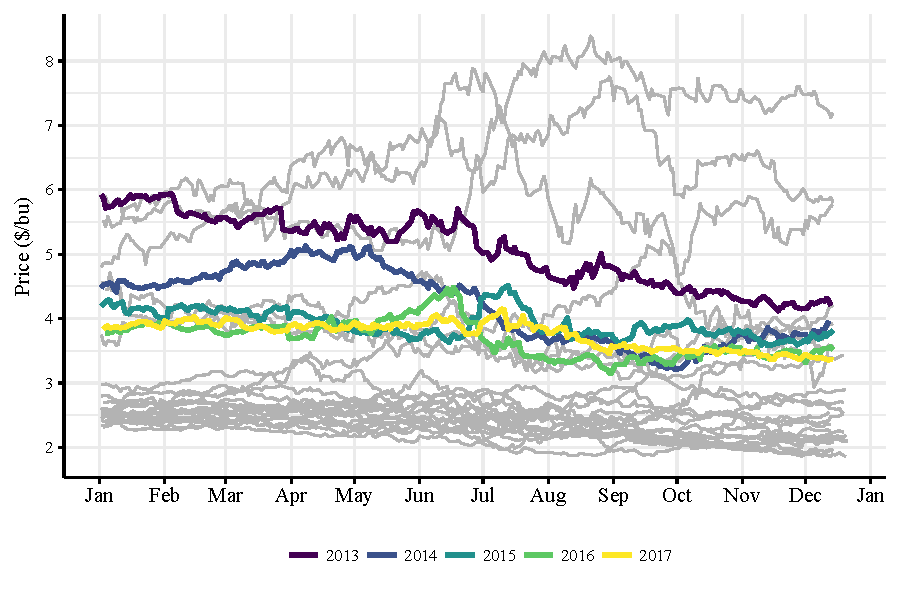
\includegraphics[width=\maxwidth]{figure/figure_corn_futures-1} 

\end{knitrout}
\end{frame}
 
%%%%%%%%%%%%%%%%%%%%%%%%%%%%%%%%%%%%%%%%%%%%%%%%%%%%%%%%%%%%%%%%%%%%%%%%%%%%%%%%%%
 
\begin{frame}{Call option premium}
\begin{knitrout}
\definecolor{shadecolor}{rgb}{0.969, 0.969, 0.969}\color{fgcolor}
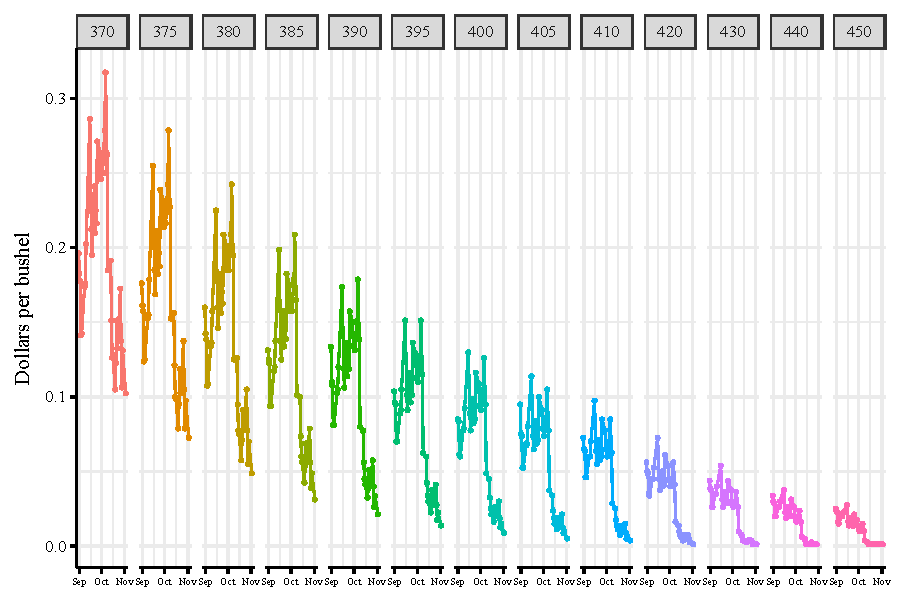
\includegraphics[width=\maxwidth]{figure/call_premium-1} 

\end{knitrout}
\end{frame}
 
%%%%%%%%%%%%%%%%%%%%%%%%%%%%%%%%%%%%%%%%%%%%%%%%%%%%%%%%%%%%%%%%%%%%%%%%%%%%%%%%%%

\begin{frame}{Put option premium}
\begin{knitrout}
\definecolor{shadecolor}{rgb}{0.969, 0.969, 0.969}\color{fgcolor}
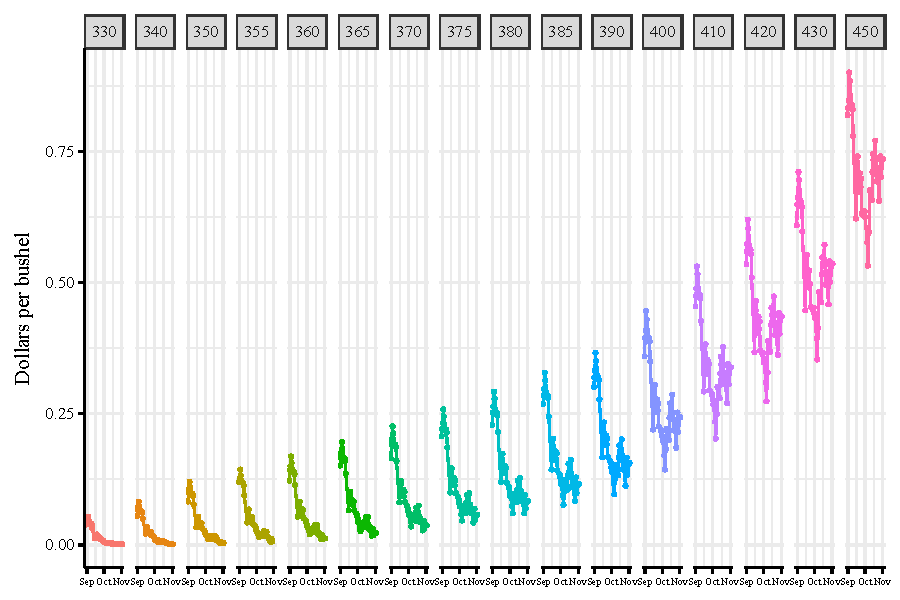
\includegraphics[width=\maxwidth]{figure/put_premium-1} 

\end{knitrout}
\end{frame}

%%%%%%%%%%%%%%%%%%%%%%%%%%%%%%%%%%%%%%%%%%%%%%%%%%%%%%%%%%%%%%%%%%%%%%%%%%%%%%%%%%

\begin{frame}{Call option intrinsic value}
\begin{knitrout}
\definecolor{shadecolor}{rgb}{0.969, 0.969, 0.969}\color{fgcolor}
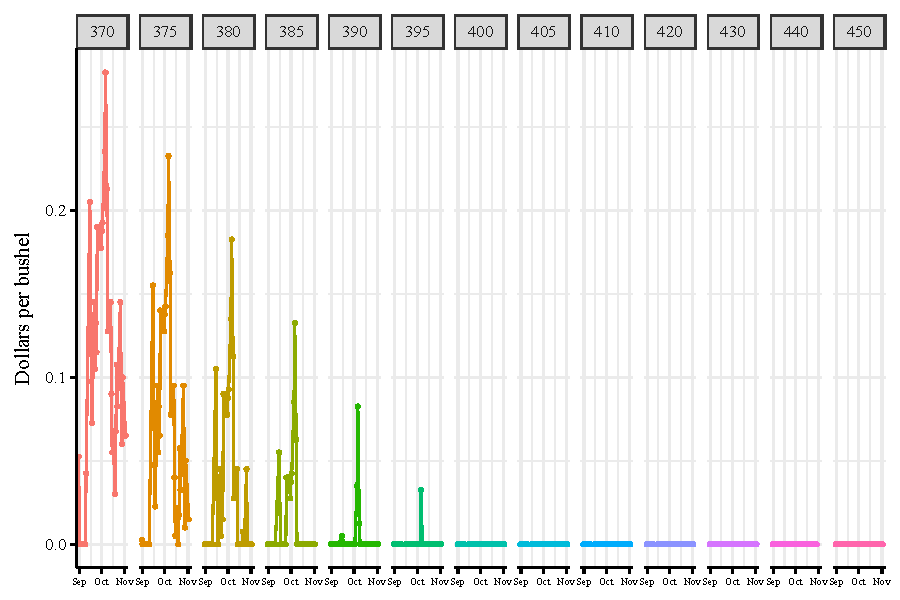
\includegraphics[width=\maxwidth]{figure/call_intrinsic-1} 

\end{knitrout}
\end{frame}

%%%%%%%%%%%%%%%%%%%%%%%%%%%%%%%%%%%%%%%%%%%%%%%%%%%%%%%%%%%%%%%%%%%%%%%%%%%%%%%%%%

\begin{frame}{Put option intrinsic value}
\begin{knitrout}
\definecolor{shadecolor}{rgb}{0.969, 0.969, 0.969}\color{fgcolor}
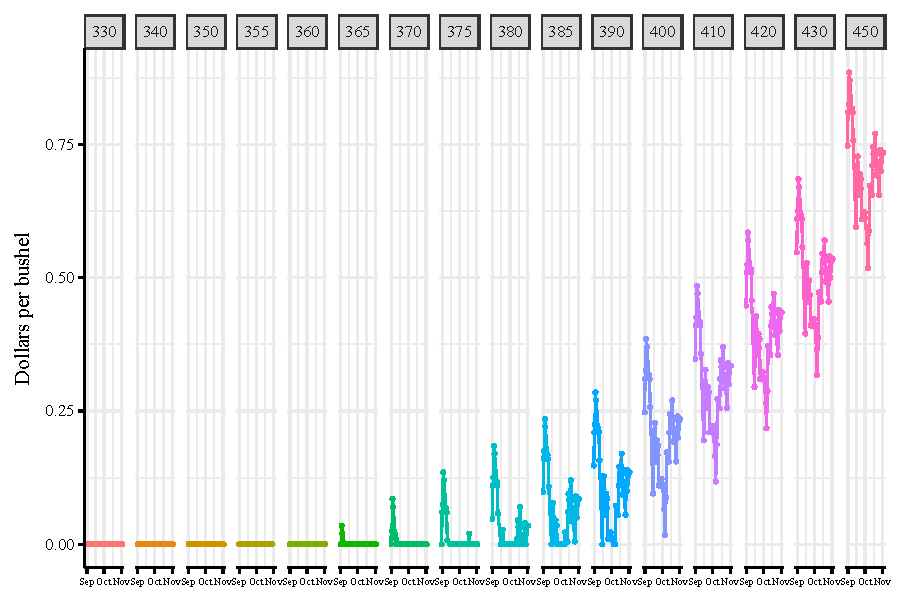
\includegraphics[width=\maxwidth]{figure/put_intrinsic-1} 

\end{knitrout}
\end{frame}

%%%%%%%%%%%%%%%%%%%%%%%%%%%%%%%%%%%%%%%%%%%%%%%%%%%%%%%%%%%%%%%%%%%%%%%%%%%%%%%%%%

\begin{frame}{Call option time value}
\begin{knitrout}
\definecolor{shadecolor}{rgb}{0.969, 0.969, 0.969}\color{fgcolor}
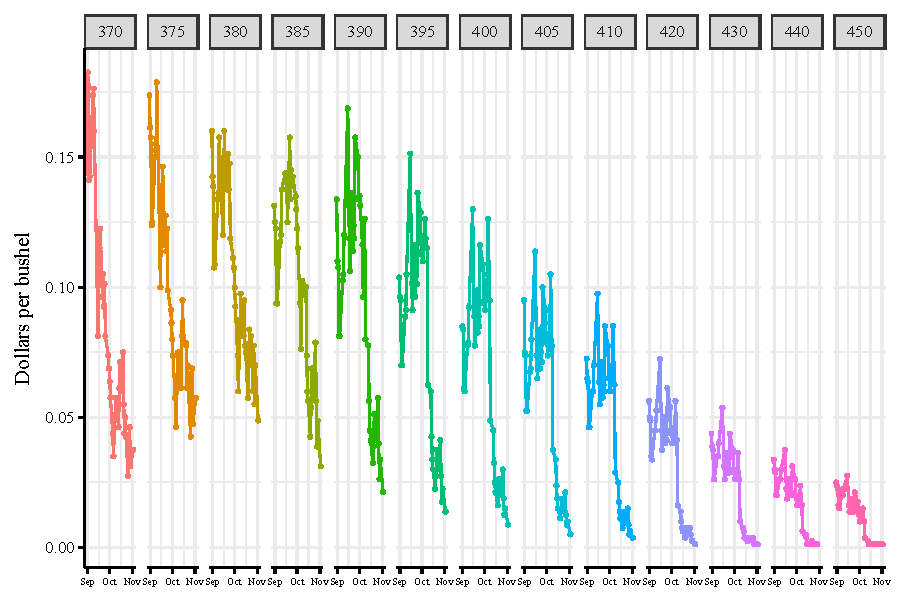
\includegraphics[width=\maxwidth]{figure/call_time-1} 

\end{knitrout}
\end{frame}

%%%%%%%%%%%%%%%%%%%%%%%%%%%%%%%%%%%%%%%%%%%%%%%%%%%%%%%%%%%%%%%%%%%%%%%%%%%%%%%%%%

\begin{frame}{Put option time value}
\begin{knitrout}
\definecolor{shadecolor}{rgb}{0.969, 0.969, 0.969}\color{fgcolor}
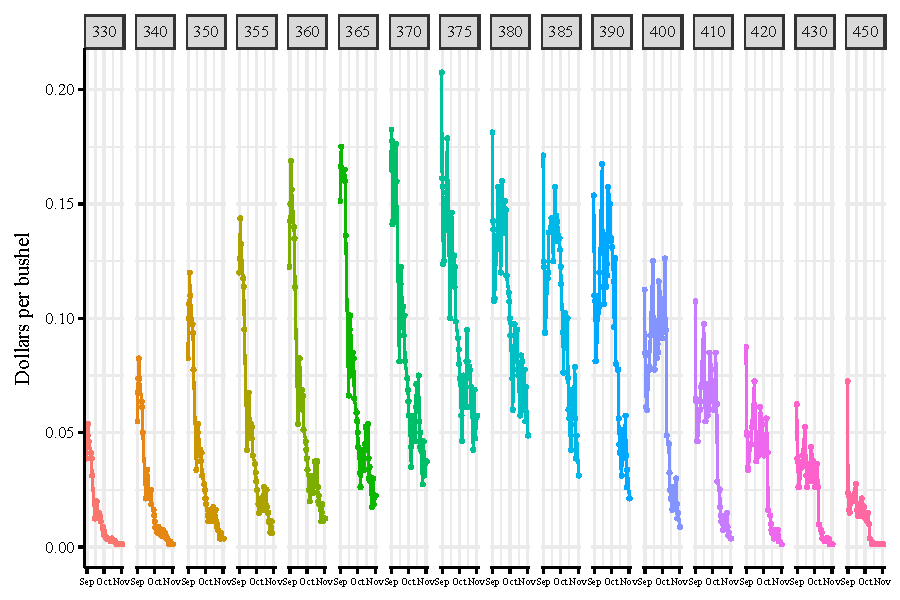
\includegraphics[width=\maxwidth]{figure/put_time-1} 

\end{knitrout}
\end{frame}

%%%%%%%%%%%%%%%%%%%%%%%%%%%%%%%%%%%%%%%%%%%%%%%%%%%%%%%%%%%%%%%%%%%%%%%%%%%%%%%%%%

\begin{frame}{Time value}
\begin{enumerate}[label=\textbullet]
  \item Some of these options are not traded very frequently.
  \item This means that the time values calculated in the previous do not always reflect the value of time alone.
  \item The corn price used for the calculations is the closing price. The last transaction for some options might have occurred quite some time before at a different corn price.
  \item This means that the time values, in the two previous graphs, are calculated with less precision.
  \item You expect the time value to decline over time.
\end{enumerate}
\end{frame}

%%%%%%%%%%%%%%%%%%%%%%%%%%%%%%%%%%%%%%%%%%%%%%%%%%%%%%%%%%%%%%%%%%%%%%%%%%%%%%%%%%

\begin{frame}{Price limits for options: call}
\begin{enumerate}[label=\textbullet]
  \item The maximum value of a call option is the price of the futures:
      \begin{enumerate}[label=-]
          \item Even if the strike price is zero, no buyer would pay more than the price of the futures.
       \end{enumerate}
  \item The minimum price of a call option is the intrinsic value, if any:
      \begin{enumerate}[label=-]
          \item If the time value equals zero, than a buyer would not pay more than the intrinsic value.
       \end{enumerate}
\end{enumerate}
\end{frame}
%%%%%%%%%%%%%%%%%%%%%%%%%%%%%%%%%%%%%%%%%%%%%%%%%%%%%%%%%%%%%%%%%%%%%%%%%%%%%%%%%%

\begin{frame}{Price limits for options: put}
\begin{enumerate}[label=\textbullet]
  \item The maximum value of a put option is the strike price:
      \begin{enumerate}[label=-]
          \item The maximum value of a put option is when the price of the futures contract equals zero.
       \end{enumerate}
  \item The minimum price of a put option is the intrinsic value, if any:
      \begin{enumerate}[label=-]
          \item If the time value equals zero, than a buyer would not pay more than the intrinsic value.
       \end{enumerate}
\end{enumerate}
\end{frame}

%%%%%%%%%%%%%%%%%%%%%%%%%%%%%%%%%%%%%%%%%%%%%%%%%%%%%%%%%%%%%%%%%%%%%%%%%%%%%%%%%%

\begin{frame}{Maximum and minimum price for options}
\begin{table}
\caption{Maximum and minimum price for options}
\scriptsize
\begin{tabular}{l c c }
  \toprule
    & Call option & Put option \\
  \midrule
  Max. price & Futures price & Strike price\\
  \addlinespace[0.075in]
  Min. price & Max[0, (futures price - strike price)] & Max[0, (strike price - futures price)]\\
  \bottomrule
\end{tabular}
\end{table}
\end{frame}

%%%%%%%%%%%%%%%%%%%%%%%%%%%%%%%%%%%%%%%%%%%%%%%%%%%%%%%%%%%%%%%%%%%%%%%%%%%%%%%%%%%%%
\section{Speculation}

\begin{frame}{Speculation using options}
\begin{enumerate}[label=\textbullet]
  \item Speculation is an attempt to profit from movements in the price of assets.
  \item Speculation using futures is relatively straightforward:
      \begin{enumerate}[label=-]
          \item The seller of a futures contract, short position, gains if the price declines.
          \item The buyer of a futures contract, long position, gains  if the price increases.
       \end{enumerate}
  \item For options, gains are directly related to the price of the underlying futures contract.
\end{enumerate}
\end{frame}

%%%%%%%%%%%%%%%%%%%%%%%%%%%%%%%%%%%%%%%%%%%%%%%%%%%%%%%%%%%%%%%%%%%%%%%%%%%%%%%%%%%%%

\begin{frame}{Definitions}
\begin{enumerate}[label=\textbullet]
    \item A \emph{bear market} is when the price of a commodity declines.
      \begin{enumerate}[label=-]
          \item If you are attacked by a bear, it will strike you DOWN with its claws.
          \item A speculator who takes a bearish position expects the price of a commodity to decline.
       \end{enumerate}
    \item A \emph{bull market} is when the price of a commodity increases.
      \begin{enumerate}[label=-]
          \item If you are attacked by a bull, it will strike you UP with its horns.
          \item A speculator who takes a bullish position expects the price of a commodity to increase.
       \end{enumerate}
\end{enumerate}
\end{frame}

%%%%%%%%%%%%%%%%%%%%%%%%%%%%%%%%%%%%%%%%%%%%%%%%%%%%%%%%%%%%%%%%%%%%%%%%%%%%%%%%%%%%%

\begin{frame}{Wall Street bull}
        \framedgraphic{Bull_Wall_Street.png}
\end{frame}

%%%%%%%%%%%%%%%%%%%%%%%%%%%%%%%%%%%%%%%%%%%%%%%%%%%%%%%%%%%%%%%%%%%%%%%%%%%%%%%%%%

\begin{frame}{Position and price expectations}
\begin{table}
\caption{Position and price expectations}
\scriptsize
\begin{tabular}{l c c }
  \toprule
    & Call option & Put option \\
  \midrule
  Buyer & Bullish & Bearish\\
  \addlinespace[0.075in]
  Seller & Neutral to bearish & Neutral to bullish \\
  \bottomrule
\end{tabular}
\end{table}
\end{frame}

%%%%%%%%%%%%%%%%%%%%%%%%%%%%%%%%%%%%%%%%%%%%%%%%%%%%%%%%%%%%%%%%%%%%%%%%%%%%%%%%%%

\begin{frame}{Why are sellers of options neutral?}
\begin{enumerate}[label=\textbullet]
    \item The seller of an option immediately receives the premium.
    \item Thus, a seller makes an immediate gain from selling the option.
    \item Future losses depend on the movement of the underlying contract.
    \item Given that losses are possible, and that underlying the option there is a futures contract, the seller of an option must have a margin account.
    \item The option may never be exercised.
\end{enumerate}
\end{frame}


%%%%%%%%%%%%%%%%%%%%%%%%%%%%%%%%%%%%%%%%%%%%%%%%%%%%%%%%%%%%%%%%%%%%%%%%%%%%%%%%%%

\begin{frame}{Payoffs from call option}
\begin{figure}[htbp]
\begin{center}
    \begin{picture}(240,180)
        %Axises and labels
        \scriptsize
        \put(0,90){\vector(1,0){240}} %x-axis
        \put(0,0){\line(0,1){180}} %y-axis
        \put(160,80){Futures price at exercise}
        \put(-5,170){\makebox(0,0){$+$}}
        \put(-5,5){\makebox(0,0){$-$}}
        \put(-5,90){\makebox(0,0){$0$}}
        %
        \thicklines
        %Call option buyer
        \color{red}
        \multiput(0,50)(5,0){16}{\line(1,0){1.5}}%Dashed line
        \put(175,145){\vector(1,1){5}}
        \multiput(80,50)(5,5){20}{\line(1,1){1.5}}%Dashed line
        \put(170,155){Call option \textcolor[rgb]{0.00,0.00,1.00}{buyer}}
        %Call option seller
        \color{black}
        \put(0,130){\line(1,0){80}}
        \put(80,130){\vector(1,-1){100}}
        \put(170,20){Call option \textcolor[rgb]{0.00,0.00,1.00}{seller}}
        %
        \multiput(80,0)(0,5){36}{\line(0,1){1.5}}%Dashed line
        %
        \put(8,5){Out of the money}
        \put(95,5){In the money}
        %
        \put(-2,70){\makebox(0,0){$\left\{\rule{0pt}{20pt}\right.$}}
        \put(-40,68){Premium}
        \put(-2,110){\makebox(0,0){$\left\{\rule{0pt}{20pt}\right.$}}
        \put(-40,108){Premium}
        \put(78,88){$\bullet$}
        \put(118,88){$\bullet$}
    \end{picture}
\vspace{0.1in}
\caption{Call option payoff line}
\end{center}
\end{figure}
\end{frame}

%%%%%%%%%%%%%%%%%%%%%%%%%%%%%%%%%%%%%%%%%%%%%%%%%%%%%%%%%%%%%%%%%%%%%%%%%%%%%%%%%%

\begin{frame}{Payoffs from put option}
\begin{figure}[htbp]
\begin{center}
    \begin{picture}(240,180)
        %Axises and labels
        \scriptsize
        \put(0,90){\vector(1,0){240}} %x-axis
        \put(0,0){\line(0,1){180}} %y-axis
        \put(160,80){Futures price at exercise}
        \put(-5,170){\makebox(0,0){$+$}}
        \put(-5,5){\makebox(0,0){$-$}}
        \put(-5,90){\makebox(0,0){$0$}}
        %
        \thicklines
        %Put option buyer
        \color{red}
        \multiput(100,50)(5,0){24}{\line(1,0){1.5}}%Dashed line
        \put(25,125){\vector(-1,1){5}}
        \multiput(100,50)(-5,5){16}{\line(-1,1){1.5}}%Dashed line
        \put(10,135){Put option \textcolor[rgb]{0.00,0.00,1.00}{buyer}}
        %
        %Put option seller
        \color{black}
        \put(100,130){\line(1,0){120}}
        \put(100,130){\vector(-1,-1){80}}
        \put(10,40){Put option \textcolor[rgb]{0.00,0.00,1.00}{seller}}

        %
        \multiput(100,0)(0,5){36}{\line(0,1){1.5}}%Dashed line
        %
        \put(18,5){In the money}
        \put(115,5){Out of the money}
        %
        \put(-2,70){\makebox(0,0){$\left\{\rule{0pt}{20pt}\right.$}}
        \put(-40,68){Premium}
        \put(-2,110){\makebox(0,0){$\left\{\rule{0pt}{20pt}\right.$}}
        \put(-40,108){Premium}
        \put(98,88){$\bullet$}
        \put(58,88){$\bullet$}

    \end{picture}
\vspace{0.1in}
\caption{Payoffs from put option} \label{fig.put_option_pay}
\end{center}
\end{figure}
\end{frame}




%%%%%%%%%%%%%%%%%%%%%%%%%%%%%%%%%%%%%%%%%%%%%%%%%%%%%%%%%%%%%%%%%%%%%%%%%%%%%%%%%%%%%
\section[References]{References}
\renewcommand\refname{References}
\def\newblock{References}
\begin{frame}[allowframebreaks]{References}
%\bibliography{R:/users/pouliot/Papers/References}
\bibliography{D:/Dropbox/Papers/References}
\end{frame}


%%%%%%%%%%%%%%%%%%%%%%%%%%%%%%%%%%%%%%%%%%%%%%%%%%%%%%%%%%%%%%%%%%%%%%%%%%%%%%%%%%%%%

\end{document}
